%%%%%%%%%%%%%%%%%%%%%%%%%%%%%%%%%%%%%%%%%
% Short Sectioned Assignment LaTeX Template Version 1.0 (5/5/12)
% This template has been downloaded from: http://www.LaTeXTemplates.com
% Original author:  Frits Wenneker (http://www.howtotex.com)
% License: CC BY-NC-SA 3.0 (http://creativecommons.org/licenses/by-nc-sa/3.0/)
%%%%%%%%%%%%%%%%%%%%%%%%%%%%%%%%%%%%%%%%%

%----------------------------------------------------------------------------------------
%	PACKAGES AND OTHER DOCUMENT CONFIGURATIONS
%----------------------------------------------------------------------------------------

\documentclass[paper=a4, fontsize=11pt]{scrartcl} % A4 paper and 11pt font size

% ---- Entrada y salida de texto -----

\usepackage[T1]{fontenc} % Use 8-bit encoding that has 256 glyphs
\usepackage[utf8]{inputenc}
%\usepackage{fourier} % Use the Adobe Utopia font for the document - comment this line to return to the LaTeX default

% ---- Idioma --------

\usepackage[spanish, es-tabla]{babel} % Selecciona el español para palabras introducidas automáticamente, p.ej. "septiembre" en la fecha y especifica que se use la palabra Tabla en vez de Cuadro

% ---- Otros paquetes ----

\usepackage{url} % ,href} %para incluir URLs e hipervínculos dentro del texto (aunque hay que instalar href)
\usepackage{amsmath,amsfonts,amsthm} % Math packages
%\usepackage{graphics,graphicx, floatrow} %para incluir imágenes y notas en las imágenes
\usepackage{graphics,graphicx, float} %para incluir imágenes y colocarlas

% Para hacer tablas comlejas
%\usepackage{multirow}
%\usepackage{threeparttable}

%\usepackage{sectsty} % Allows customizing section commands
%\allsectionsfont{\centering \normalfont\scshape} % Make all sections centered, the default font and small caps

\usepackage{fancyhdr} % Custom headers and footers
\pagestyle{fancyplain} % Makes all pages in the document conform to the custom headers and footers
\fancyhead{} % No page header - if you want one, create it in the same way as the footers below
\fancyfoot[L]{} % Empty left footer
\fancyfoot[C]{} % Empty center footer
\fancyfoot[R]{\thepage} % Page numbering for right footer
\renewcommand{\headrulewidth}{0pt} % Remove header underlines
\renewcommand{\footrulewidth}{0pt} % Remove footer underlines
\setlength{\headheight}{13.6pt} % Customize the height of the header

\numberwithin{equation}{section} % Number equations within sections (i.e. 1.1, 1.2, 2.1, 2.2 instead of 1, 2, 3, 4)
\numberwithin{figure}{section} % Number figures within sections (i.e. 1.1, 1.2, 2.1, 2.2 instead of 1, 2, 3, 4)
\numberwithin{table}{section} % Number tables within sections (i.e. 1.1, 1.2, 2.1, 2.2 instead of 1, 2, 3, 4)

\setlength\parindent{0pt} % Removes all indentation from paragraphs - comment this line for an assignment with lots of text

\newcommand{\horrule}[1]{\rule{\linewidth}{#1}} % Create horizontal rule command with 1 argument of height

\graphicspath{ {./images/} }
\usepackage{subcaption}
\usepackage[hidelinks]{hyperref}
\usepackage{soul}


%----------------------------------------------------------------------------------------
%	TÍTULO Y DATOS DEL ALUMNO
%----------------------------------------------------------------------------------------

\title{	
\normalfont \normalsize 
\textsc{\textbf{Técnicas de los Sistemas Inteligentes (2019)} \\ Doble Grado en Ingeniería Informática y Matemáticas \\ Universidad de Granada} \\ [25pt] % Your university, school and/or department name(s)
\horrule{0.5pt} \\[0.4cm] % Thin top horizontal rule
\huge Memoria Práctica 1 \\ % The assignment title
\horrule{2pt} \\[0.5cm] % Thick bottom horizontal rule
}

\author{Ignacio Aguilera Martos \\ Luis Balderas Ruiz} 
 % Nombre y apellidos 


\date{\normalsize\today} % Incluye la fecha actual

%----------------------------------------------------------------------------------------
% DOCUMENTO
%----------------------------------------------------------------------------------------

\begin{document}

\maketitle % Muestra el Título

\newpage %inserta un salto de página

\tableofcontents % para generar el índice de contenidos

\listoffigures

\newpage

\section{Introducción}

La práctica propuesta, encuadrada en GVG-IA, más concretamente el videojuego Boulder Chase, tiene como objetivo diseñar un comportamiento inteligente del avatar protagonista del juego para conseguir 10 gemas (aunque se puede comprobar que con 9 es suficiente) evitando el contacto con escorpiones y murciélagos, a la vez que se esquivan piedras móviles. Cuando se tienen las gemas necesarias, se debe salir por el portal para completar el mapa. \\

A pesar de no ser un problema de planificación al uso (tal y como vemos en las prácticas siguientes y en teoría), nuestro enfoque se basa en planificar, a corto y medio plazo, cuáles son las gemas más interesantes a coger en función de la dificultad/peligrosidad que plantean y cuál es el camino idóneo para ello. Esta planificación se divide en dos estadios: planificación a alto nivel, en la que se decide qué gemas coger y en qué orden; y una planificación a bajo nivel, donde se establece el camino a seguir y sus posibles alteraciones consecuencia de la detección de enemigos. En el presente documento explicamos el comportamiento con detalle.

\section{Planificación a alto nivel}

El mundo de Boulder Chase se encuadra en un mapa con los bordes delimitados por muros y, en su interior, encontraremos casillas vacías, con rocas, tierra, enemigos, gemas y un portal. Si jugáramos manualmente, nuestro criterio nos conduciría a elegir como objetivo aquellas gemas más cercanas en las que se garantiza, de una manera u otra, que los enemigos no nos alcanzan. Además, teniendo en cuenta que el avatar tiene la capacidad de mover piedras, podríamos explorar nuevas zonas del mapa (a priori inaccesibles) para así coger gemas extra. Cuando la barra de objetivos se completa (con 9-10 gemas), el avatar debe escapar por el portal para completar el mapa. Todo ello se debe conseguir con dos restricciones de tiempo: la primera es que se tienen 2000 ticks para completar el mapa; la segunda es que cada acción debe llevarse a cabo en menos de 40 ms. De la segunda restricción nos ocuparemos más adelante. Por el momento, debemos establecer un criterio de elección de gemas para ser completado en menos de 2000 ticks.  \\

Teniendo todo esto en mente, nuestro avatar establece una prioridad entre la gemas en función de los siguientes aspectos:

\begin{itemize}
	\item La gema es accesible (existe un camino disponible entre el avatar y la gema), no se encuentra bajo una piedra y está fuera del alcanze de un enemigo. A este conjunto de piedras las llamamos \textit{gemas fáciles}.
	\item La gema requiere mover piedras para ser capturada pero no está en el entorno de un bicho. Este caso es amplio, por lo que hemos elegido algunos casos particulares que cubren las necesidades. Lo trataremos a continuación con más profundidad.
	\item La gema es accesible pero en el camino hay que lidiar con enemigos, en otras palabras, el camino que lleva al avatar hasta la gema pasa por una zona donde un enemigo se mueve (incide en el entorno de un enemigo). Como consecuencia, habrá que esquivarlo de alguna manera y, a partir de ese momento, el espacio donde el enemigo puede moverse aumenta. Este es el caso más complejo. En la planificación a bajo nivel explicamos con detalle qué comportamiento tiene el avatar cuando detecta un enemigo cerca.
\end{itemize} 

Como es lógico, intentamos conseguir el máximo número de gemas fáciles y que requieren mover piedras para así evitar, en la medida de lo posible, enfrentarnos a enemigos. Así conseguimos maximizar la ratio de victorias en los mapas. No obstante, existen mapas, como el número 0, que requieren \textit{luchar} contra enemigos, por lo que hemos dedicado un gran esfuerzo en detectarlos y esquivarlos de forma eficiente y eficaz.

\subsection{Gemas fáciles}

Utilizando la funcionalidad \textit{getResourcesPositions} de GVG-IA obtenemos la lista de gemas y comprobamos aquellas que son accesibles y no están en el entorno de un enemigo (no están en el interior ni en la frontera de la zona donde un enemigo se puede mover) y la ordenamos teniendo en cuenta la distancia Manhattan, es decir, la primera que asignamos es la que está más cerca de la posición inicial y, a continuación, la siguiente será la más cercana a la gema primera. De esa forma, garantizamos el camino más eficiente. \\

Nos interesaba controlar si el avatar pasa demasiado tiempo intentando alcanzar una gema. Por ello, controlamos si se queda bloqueado por medio de una variable numérica y si esa variable supera 50, la gema objetivo pasa a ser la última y se centra en la siguiente.

\subsection{Gemas que requieren mover piedras}

Como hemos comentado antes, hay una gran cantidad de casos en los que es necesario mover piedras para alcanzar una gema. Muchas de ellas son complejas, por lo que hemos elegido un conjunto de 5 casos que garantizan la adquisición de gemas necesarias para terminar los mapas. En la siguiente imagen mostramos los casos elegidos:
 
\begin{figure}[H] %con el [H] le obligamos a situar aquí la figura
	\centering
	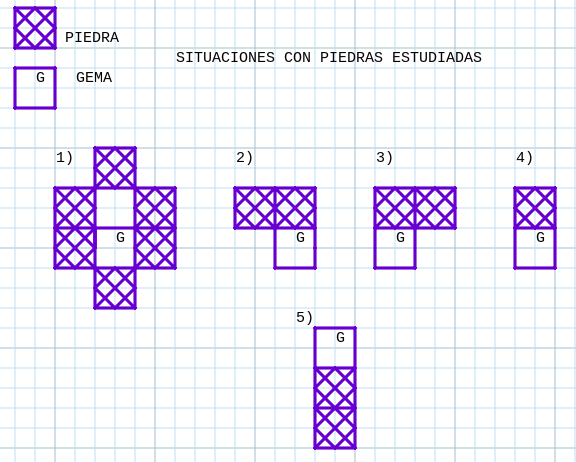
\includegraphics[scale=0.6]{piedras.png}  %el parámetro scale permite agrandar o achicar la imagen. En el nombre de archivo puede especificar directorios
	\caption{Casos de piedras consideradas para mover} 
	\label{fig:piedras}
\end{figure}

En el primer caso, es necesario que las casillas a izquierda o derecha de la piedra en las dos filas siguientes sean disponibles, para así poder tirarla. El segundo y tercer caso, análogos, se basan en coger la gema antes de que caiga la piedra (tarda 3 ticks en caer). De la misma manera, el cuarto caso. Por último, contemplamos la posibilidad de tirar una hilera de piedras para acceder a una gema situada sobre ellas. \\

Teniendo en mente los casos en los que contemplamos mover piedras, el avatar contiene una lista con las gemas que son de este tipo y trata de cogerlas cuando ya no queda ninguna gema fácil a la que acudir. De nuevo, si percibimos sensación de bloqueo, la gema actual pasa a ser la última a la que acude.

\subsection{Gemas y contacto con enemigos}

Cuando ya no quedan gemas fáciles y se han obtenido todas las gemas con rocas descritas en la sección anterior, sólo queda lidiar con enemigos. En los apartados anteriores, el avatar no podía generar caminos que pasaran por entornos de enemigos (la planificación a bajo nivel señalaba que esas casillas eran inaccesibles) de forma que se establecía un 'cordón sanitario' alrededor de los enemigos. Así, la planificación a bajo nivel no encontraba ningún camino que diera acceso a gemas con riesgo de enemigo. Cuando ya no quedan más gemas de los apartados anteriores, ese cordón se deshabilita de forma que ya si existan caminos. El éxito en este caso pasa por diseñar un buen sistema que permita al avatar esquivar a los enemigos. Nosotros hemos desarrollado dos estrategias (una de ellas reactiva) y una forma concreta de vigilar el entorno. Serán explicadas en la siguiente sección.

\section{Planificación a bajo nivel}

La planificación a bajo nivel se encarga de encontrar los caminos a las gemas de la manera más eficiente. Para ello, utilizamos el algoritmo $A^*$ con ciertas peculiaridades. Por otra parte, en el recorrido de los caminos es usual encontrar enemigos, por lo que hemos diseñado un sistema que los esquiva.

\subsection{Construcción de caminos con $A^*$}

$A^*$ es el algoritmo utilizado por antonomasia para resolver problemas heurísticos. En este caso, a través de la distancia Manhattan, conseguimos encontrar el camino óptimo (minimizando la distancia). Sin embargo, retomando la restricción temporal de 40 ms por acción, $A^*$ podría tardar demasiado en encontrar el camino entre dos casillas. Por este motivo, hemos contemplado la posibilidad de almacenar el estado del algoritmo (lista de nodos abiertos y cerrados, nodo actual) cuando se sobrepasa un tiempo determinado, devolver una acción nula y continua el procedimiento en el siguiente turno. Así, en un número finito de turnos, se calcularía un camino óptimo. Otra opción sería calcular caminos óptimos parciales, aunque experimentalmente hemos determinado que el comportamiento es mucho más errático. Por otra parte, una buena implementación, usando estructuras de datos convenientes y métodos eficientes de comparación de nodos (vía \textit{hashCode}) hace que prácticamente siempre se encuentren los caminos completos en un único turno. Hay que tener en cuenta que $A^*$ considera que una casilla es accesible si no cumple:

\begin{enumerate}
	\item La casilla es un muro
	\item La casilla es una roca
	\item La casilla tiene una roca encima
	\item La casilla contiene un enemigo
\end{enumerate}

 Una vez calculado el camino por casillas accesibles, el avatar mantiene una lista de acciones que va ejecutando hasta llegar al destino. Cuando la lista de acciones llega a cero, accede a las estructuras de gemas generadas en la planificación a alto nivel (fáciles, por piedras o contra enemigos, según toque) y calcula un nuevo camino. 

\subsection{Esquivando enemigos}

Cuando $A^*$ construye un camino, el avatar lo recorre fielmente. Si hay un enemigo cerca accesible, hay una gran probabilidad de que el enemigo y el avatar choquen y quedemos descalificados. Por tanto, es necesario saber reaccionar ante la presencia de un enemigo, esquivarlo de forma reactiva o huir. Para poder reaccionar, es necesario detectarlo con al menos una distancia de tres casillas, ya que si se quiere escapar avanzando en sentido contrario, dar un paso hacia atrás requeriría dos acciones (cambiar el sentido y avanzar). Estando a tres casillas, el enemigo es incapaz de alcanzar al avatar en dos turnos. Para conseguirlo, dotamos al personaje con la capacidad de revisar, dependiendo de la orientación, las siguientes casillas en busca de enemigos (en adelante, los conos de visión):

\begin{figure}[H] %con el [H] le obligamos a situar aquí la figura
	\centering
	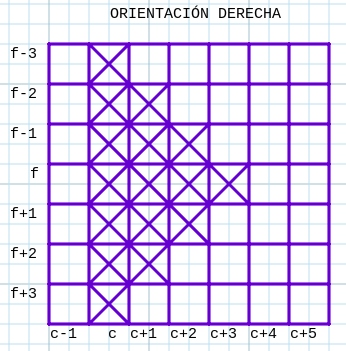
\includegraphics[scale=0.6]{or-der.png}  %el parámetro scale permite agrandar o achicar la imagen. En el nombre de archivo puede especificar directorios
	\caption{Casillas a revisar con orientación hacia la derecha} 
	\label{fig:orientación-dcha}
\end{figure}

\begin{figure}[H] %con el [H] le obligamos a situar aquí la figura
	\centering
	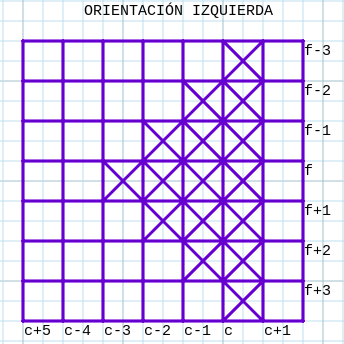
\includegraphics[scale=0.6]{or-izq.png}  %el parámetro scale permite agrandar o achicar la imagen. En el nombre de archivo puede especificar directorios
	\caption{Casillas a revisar con orientación hacia la izquierda} 
	\label{fig:orientación-izq}
\end{figure}

\begin{figure}[H] %con el [H] le obligamos a situar aquí la figura
	\centering
	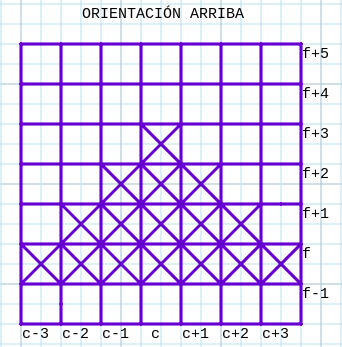
\includegraphics[scale=0.6]{or-arr.png}  %el parámetro scale permite agrandar o achicar la imagen. En el nombre de archivo puede especificar directorios
	\caption{Casillas a revisar con orientación hacia arriba} 
	\label{fig:orientación-arr}
\end{figure}

\begin{figure}[H] %con el [H] le obligamos a situar aquí la figura
	\centering
	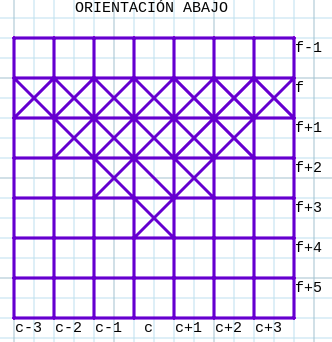
\includegraphics[scale=0.6]{or-abaj.png}  %el parámetro scale permite agrandar o achicar la imagen. En el nombre de archivo puede especificar directorios
	\caption{Casillas a revisar con orientación hacia abajo} 
	\label{fig:orientación-abaj}
\end{figure}

Una vez detectada la presencia de un enemigo en el cono de visión, se produce el conjunto de acciones para esquivar. El comportamiento es aleatorio. Más de un 75\% de las veces, el avatar escapa hacia el punto de inicio, el portal o el punto más alejado de los dos anteriores. Con menos de un 25\% de probabilidad, buscamos una casilla accesible que maximiza la distancia al enemigo más cercano. De esta manera, conseguimos alejarnos y, a la vez, abrimos mapa de forma que el enemigo pueda moverse y no permanezca siempre en el mismo entorno. Puede darse el caso, incluso, de que dos enemigos del mismo tipo (murciélago o escorpión) interaccionen entre sí, eliminándose y generando una nueva gema. Por tanto, resulta muy interesante facilitarles el movimiento por todo el mapa, aumentando la probabilidad de que se autodestruyan. Así, es posible conseguir vía libre hacia las gemas que antes estaban inaccesibles por la presencia del enemigo. Además, si en el camino de huida encontrara otro enemigo, no tendría sentido volver a activar el mismo comportamiento de huida. Por este motivo, hemos desarrollado también un comportamiento reactivo en el que el avatar se mueve en sentido contrario al movimiento que venía realizando (por ejemplo, si caminaba hacia a la izquierda, el comportamiento reactivo introduce en la lista de acciones dos nuevas: derecha y derecha, generando el cambio de sentido y el paso atrás).

\end{document}
